\normaltrue \difficilefalse \tdifficilefalse
\correctiontrue

%\UPSTIidClasse{11} % 11 sup, 12 spé
\newcommand{\UPSTIidClasse}{12}

\exer{Train simple $\star$ \label{C2:06:21}}
\setcounter{numques}{0}
\UPSTIcompetence[2]{A3-05}
\UPSTIcompetence[2]{C2-06}
\index{Compétence C2-06}
\index{Train d'engrenages simple}
\ifcorrection
\else
\textbf{Pas de corrigé pour cet exercice.}
\fi

\ifprof
\else
Soit le train d'engrenages suivant. 
\begin{center}
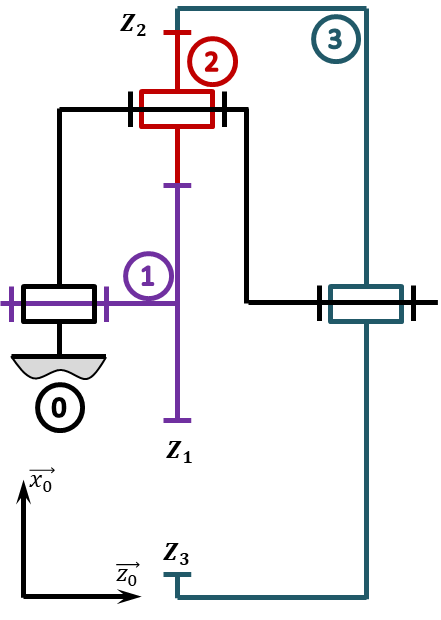
\includegraphics[width=.7\linewidth]{21_01}
\end{center}
\fi


\question{Tracer le graphe des liaisons.}
\ifprof
\else
\fi

\question{Déterminer $\dfrac{\omega_{3/0}}{\omega_{1/0}}$ en fonction du nombre de dents des roues dentées.}
\ifprof ~\\
On a $\dfrac{\omega_{3/0}}{\omega_{1/0}}=-\dfrac{Z_1}{Z_3}$.
\else
\fi

\question{Donner une relation géométrique entre $Z_1$, $Z_2$ et $Z_3$ permettant de garantir le fonctionnement du train d'engrenages.}
\ifprof~\\
On a $Z_3 = 2Z_2 + Z_1$.
\else
\fi

\ifprof
\else
\begin{flushright}
\footnotesize{Corrigé  voir \ref{C2:06:21}.}
\end{flushright}%
\fi